% !TEX encoding = UTF-8 Unicode
% !TEX root = ../Saunkin.tex

\chapter{Related work and systems} \label{c2:related-work}

The analysis of scientific citations has been an active area of research within the field of bibliometrics \snote{add some refs}.
A number of metrics, data sources, and analytical approaches have been developed to assess the impact of publications and researchers \snote{add some refs}.

This chapter presents an overview of the fundamental concepts and existing systems relevant to citation analysis.

\section{Data sources} \label{sec:data-sources}

Citation data is obtained from specialized search services that index scientific publications and their references \snote{add some refs}.
These systems allow users to search for publications, track citation counts, and explore connections between works.

At the same time, these systems present several limitations \snote{are there paper that also point this? If yes please add. }.
Access to data is often restricted or rate limited, metadata is inconsistent across articles, and authors are not uniquely defined across data sources and publications.

To compare the sources, we can define a few aspects that matter for citation analysis: method of access, cost, extent and scope of coverage, data structure (especially whether the citing publications are treated as a first-class citizen), author identification.

Table~\ref{tab:data-sources} summarizes a few sources along these aspects.

\snote{Move tables/figure closer to their first reference. Also always use }\verb=\begin{table}[tb]=\snote{. I fixed the following table, fix the others as well.}


\begin{table}[tb]
\label{tab:data-sources}
\centering
\footnotesize
\setlength{\tabcolsep}{4pt}
\begin{tabular}{p{2.3cm} p{2.4cm} p{3.0cm} p{2.0cm} p{2.8cm}}
\hline
Source & Access & Coverage & Citations & Author data \\
\hline
\textsf{Google Scholar} & No public API; via paid proxy & Largest; all disciplines & Yes, via proxy & Profile ID; names as text \\
\textsf{OpenAlex} & Open API, free key & About 271M works & Yes & Author IDs; name search \\
\textsf{Semantic Scholar} & Open API, free key (1 req/s) & Over 200M papers; 2B citations & Yes & Author IDs; name search \\
\textsf{CrossRef} & Open API, free & Over 180M \textsf{DOI} records & Count only & No author IDs \\
\textsf{OpenCitations} & Open API and dumps, free & Over 2B citation links & Yes & \textsf{ORCID} only \\
\textsf{DBLP} & Open API and dump, free & 6.6M works; CS only & No & Strong disambiguation \\
\textsf{Scopus} & Paid subscription & About 90M curated records & Yes & Scopus author IDs \\
LLM & Model query & Broad but unverifiable & Unreliable & No identifiers \\
\hline
\end{tabular}
\caption{Comparison of the main citation data sources}
\end{table}


\begin{itemize}
    \item \textsf{Google Scholar}\footnote{\url{https://scholar.google.com}} has the widest coverage of all sources across every domain. \snote{do note leave space before a footnote, deleted it. Change everywhere!}
    It offers no structured interface and actively blocks automated access.

There is a number of third-party services, such as \textsf{SerpApi}~\footnote{\url{https://serpapi.com}}, that scrape \textsf{Google Scholar} pages on demand to provide an interface to return structured data.
    These services supply a fleet of devices to automatically handle robot detection, IP rotation, solve Captcha challenges, and avoid other traps, to reliably extract data from the pages.
    They charge a fee per request.
    These services inherit the coverage and specifics of \textsf{Google Scholar} (identify authors by profile page and expose contribution lists as plain comma-separated text).
    Some of these services provide an interface to collect the citing publications (exposed by \textsf{Google Scholar}).
    \item \textsf{OpenAlex}~\footnote{\url{https://openalex.org}} indexes about 271 million works and 213 million authors, and returns each publication together with its author list and its citing publications, so a single source can satisfy every kind of request.
    The access is provided via Application Programming Interface (API).
    The throughput is limited to ten requests per second.
    \item \textsf{Semantic Scholar}~\footnote{\url{https://www.semanticscholar.org}} holds more than 200 million papers and over two billion citations with a similar structure.
    The access is provided via Application Programming Interface (API).
    The throughput is limited to one request per second, while retrieving long citation lists requires many sequential requests.
    \item \textsf{CrossRef}~\footnote{\url{https://www.crossref.org}} provides high-quality metadata and author order for any publication that has a registered Digital Object Identifier (\textsf{DOI}).
    It reports only the number of citations rather than the list of citing publications, and exposes no author identifier.
    \item \textsf{OpenCitations}~\footnote{\url{https://opencitations.net}} aggregates more than two billion open citation links and can be downloaded in full.
    It can be queried only by identifier and offers no search by author name.
    \item \textsf{DBLP}~\footnote{\url{https://dblp.org}} provides accurate author disambiguation.
    It is limited to computer science and holds no citation links of its own.
    \item \textsf{Scopus}~\footnote{\url{https://www.scopus.com}} is a curated commercial database with high-quality metadata, stable author identifiers, and native citation retrieval.
    It requires a paid institutional subscription and covers a narrower set of journals.
    \item Large Language Models (LLM) can also be asked to list the publications of an author or the citations of a paper.
    These answers are not reliable, and they provide no stable author identifiers.
\end{itemize}

The largest source \snote{say which is?} is the hardest to access, the open sources differ in coverage \snote{say which are?} and in the data they expose, and the most curated source \snote{say which is?} is not freely available.
The sources selected for this work, and the reasons for the selection, are discussed with the implementation in Section~\ref{sec:providers}.

%\snote{The above might be true, but why they affect us. Remember the problem is self/external citation distinction. In any case you do not provide solutions for inconsistent data. You use existing meta data, right?}
%\enote{I just present the existing systems. It's the current state of things, data sources are not all equal.}
%\enote{ID incostistency, insufficient data parity, difficulty matching the authors, limit rated access - all these aspects will become issues down the road of this investigation.}
%\enote{The software I will create as part of this investigation, I will have to justify the preference of one of the data source over another (it might be due to the availability of papers on a data source), provide a solution for author matching, and a way around throttling.}

\snote{It flows OK. You could add more if needed. You may use LLM polish and extend. Do not use it to write it though and do not overdo it. We use turn-it-in to check the final thesis. It is obligatory.}

\section{Existing approaches} \label{sec:existing-approaches}

Existing approaches to citation analysis primarily rely on the aggregation and examination of citation relationships between publications.

A common representation models publications as nodes in a graph, with directed edges indicating citation relationships.
This representation enables the application of graph-based methods to quantify influence among the scientific publications~\cite{Boyack2005, Chronis2021, Chronis2020}.

\snote{
Cite also the following. 
\begin{itemize}
\item
Pantelis Chronis, Dimitrios Skoutas, Spiros Athanasiou, Spiros Skiadopoulos:
Link Prediction in Bibliographic Networks. Predicting the Dynamics of Research Impact 2021: 271-290
\url{https://dblp.uni-trier.de/rec/books/sp/21/Chronis0AS21.html?view=bibtex}.
\item
Pantelis Chronis, Dimitrios Skoutas, Spiros Athanasiou, Spiros Skiadopoulos:
Link Prediction in Bibliographic Networks. ADBIS/TPDL/EDA Workshops 2020: 335-340
\url{https://dblp.uni-trier.de/rec/conf/adbis/ChronisSAS20.html?view=bibtex}
\end{itemize}
Let me get some citations....
}

In addition to trivial citation counts, other metrics have been proposed to evaluate research impact, such as the \textsf{Hirsch index} (h-index)~\cite{Hirsch2005}, which attempts to capture both productivity and citation influence.

These approaches form the base of many existing citation analysis systems and are commonly used in the evaluation of scientific output.

\section{Research on self-citation} \label{sec:research-on-self-citation}

Self-citation has been discussed in the context of bibliometrics to a limited degree.
It is generally defined as a citation where at least one author appears in both the citing and cited publications~\cite{Glnzel2003BIBLIOMETRICSAA, Fowler2007, R2008ImpactReinforcing}.
Self-citations may occur naturally when researchers build upon their own previous work.
However, excessive self-citation can artificially inflate citation-based metrics and distort the perceived impact of a publication or researcher~\cite{Fowler2007, R2008ImpactReinforcing}.

Several studies have highlighted the importance of distinguishing self-citations from external citations when evaluating scientific impact.
Nevertheless, definitions and methodologies vary across studies, and many systems do not provide explicit or consistent classification~\cite{Glnzel2003BIBLIOMETRICSAA, Costas2010}.

Recent work has focused specifically on the impact of self-citations.
For example, Fiorillo~\cite{Fiorillo2024} introduces the Fi-score, a metric designed to assess the influence of self-citations on academic impact.

Some academic databases also recognize the importance of distinguishing self-citations from external citations.
For instance, \textsf{Scopus}~\footnote{\url{https://https://www.scopus.com/}} platform allows to filter out self-citations at the author level.
While the algorithm followed in each case is not always well understood, the availability of these metrics indicates that self-citation is considered as a factor in the evaluation of scientific impact.
This observation supports the need for explicit definition and transparent methodology in identifying and classifying self-citations.

\begin{figure}
    \centering
    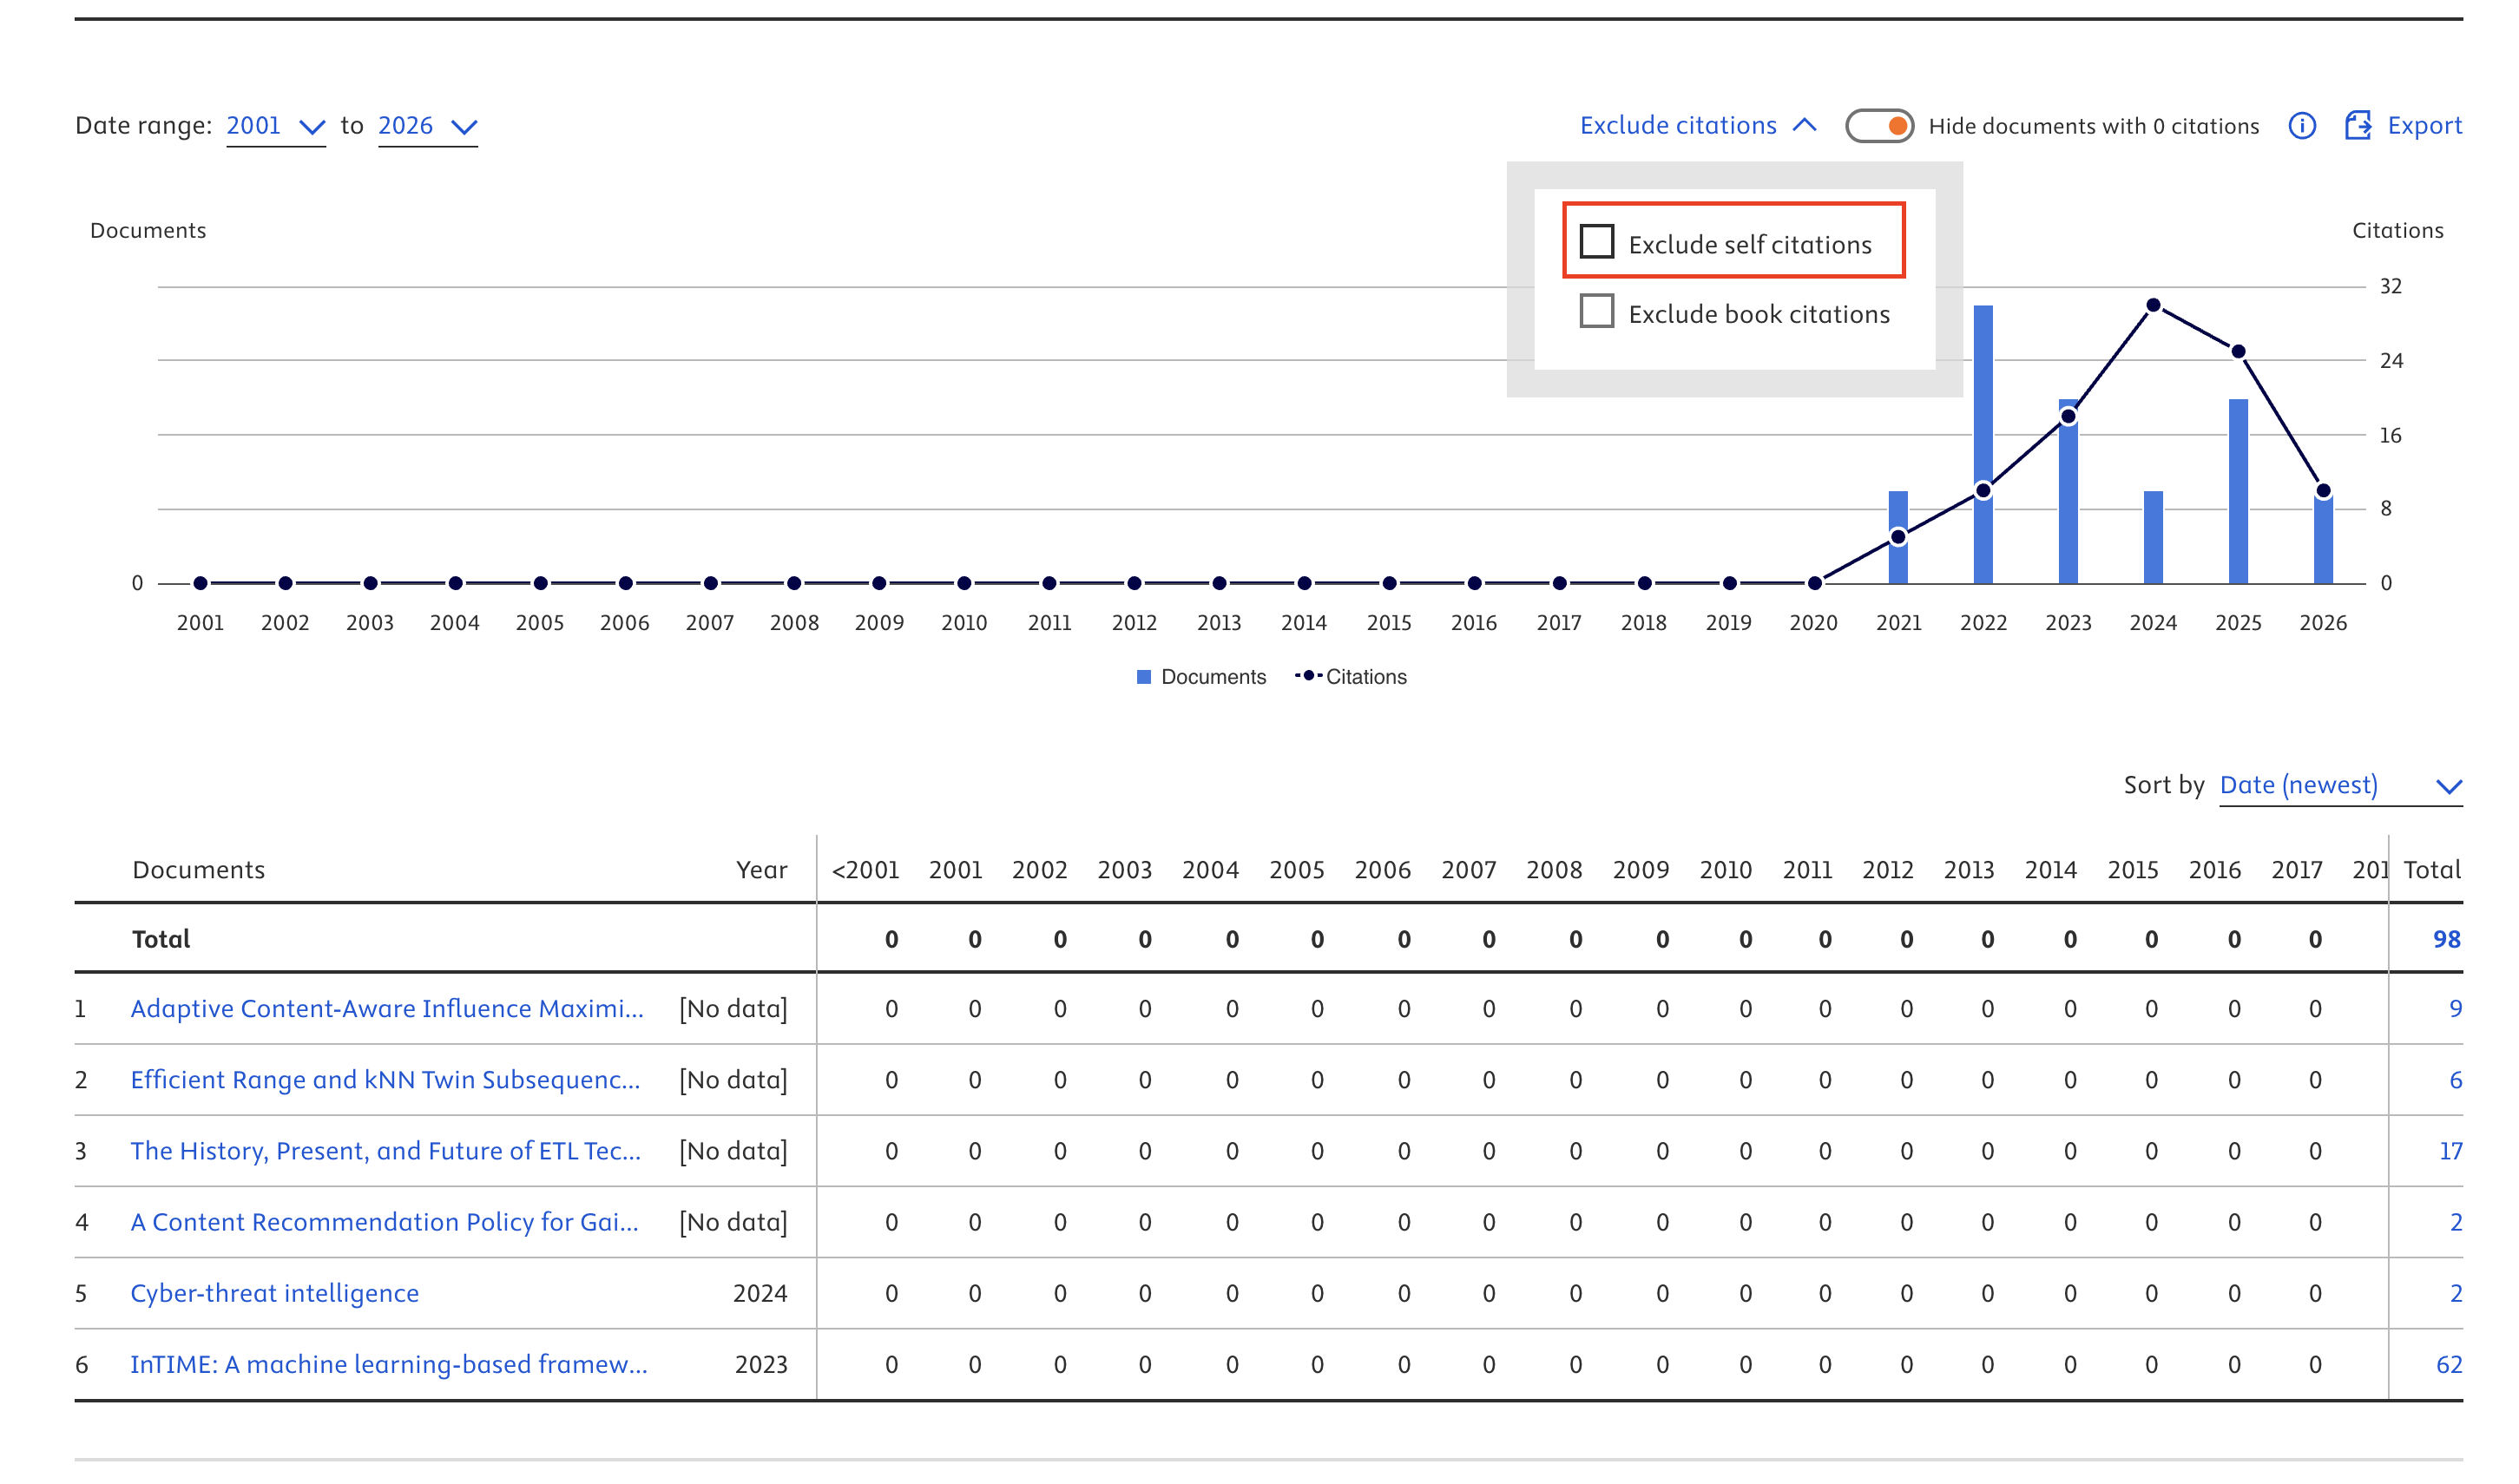
\includegraphics[width=10cm]{include/fig-scopus-2}
    \caption{Scopus interface allows to remove self-citations from the metrics}
    \label{fig:scopus-ui}
\end{figure}

\snote{You make too small paragraphs. An empty line in \LaTeX separates paragraphs. Typically, I use a single line for a paragraphs (despite the fact that intelij complains. You do not have to do like me. Yet a paragraph should have many sentences of a coherent content. You typically break the coherent content into many paragraphs. I corrected some, still keep this in mind.}
\enote{I find dense paragraphs harder to read. But I obviously can adapt and will do as you suggest.}
